
\documentclass[runningheads]{llncs}
\usepackage{graphicx}
\usepackage{apacite}
\usepackage{float}
\usepackage{listings}
\lstset{
  basicstyle=\ttfamily,
  columns=fullflexible,
  frame=single,
  breaklines=true,
  postbreak=\mbox{\textcolor{red}{$\hookrightarrow$}\space},
}
\usepackage{float}
\usepackage[table]{xcolor}
\usepackage[toc,page]{appendix}
\usepackage{ucs}
\usepackage[utf8x]{inputenc}

\usepackage{hyperref}
\hypersetup{
	colorlinks=true,
	linkcolor=blue,
	filecolor=magenta,      
	urlcolor=cyan,
}

\usepackage[slovene]{babel}
\selectlanguage{slovene}

\lstset{
    breaklines=true,
    breakatwhitespace=true,
    inputencoding=utf8,
    extendedchars=false,
}

\renewcommand{\baselinestretch}{1.2} % za boljšo berljivost večji razmak
\renewcommand{\appendixpagename}{\normalfont\Large\bfseries{Appendix}}

\begin{document}

\title{Seminarska naloga}
\subtitle{Implementacija algoritma za grupiranje in določanja vodja grupe}

\author{Danijel Maraž, Nejc Rebernik}

\institute{Fakulteta za Računalništvo in Informatiko UL
\email{dm9929@student.uni-lj.si}\\
}

\maketitle             

\begin{abstract}
The article covers the work done in the scope of the seminar assignment as part of the subject wireless sensor networks.

\keywords{Raft nRF24LO1 Leader Consensus Wemos ESP}
\end{abstract}

\section{Uvod}
Cilj projekta je bila implementacija algoritma za določanje vodje gruče brezžičnih naprav. Razvoj in testiranje sva opravljala na ploščici z WEMOS D1 mini kontrolerjem in modulom za komuniciranje nRF24L01. Na ploščici so bili nameščeni še drugi moduli, ki pa jih v obsegu najinega razvoja nisva uporabila. Modul nRF24L01 sprejema in oddaja na frekvenci 2.4GHz z maksimalno hitrostjo prenosa do 2Mbps. Majhne velikosti sporočil uporabljenih v komunikaciji in glede na to relativno velika podatkovna pretočnost sta omogočala hiter razvoj in testiranje ter skalabilnost. Za določanje vodje v gruči sva implementirala protokol RAFT. Programska koda je napisana v jeziku C++ s knjižnico za upravljanje s komunikacijskim modulom nRF24L01.

\section{Splošna struktura}
Odločila sva se, da ne bova imela več kot ene verzije kode in da se bo vsaka naprava lahko priključila na najino omrežje. Posledično je koda že sama po sebi zelo univerzalna, saj vsebuje vse kar napravi omogoča, da opravlja vse vloge RAFT protokola. Osnoven tok dogodkov sestoji iz aktivacije naprave in pogona \textit{LR\_task} in \textit{election\_task} opravil. \textit{LR\_task} opravilo je namenjeno poslušanju aktivnosti na omrežju, ter hkrati pošiljanju sporočil, ko je to potrebno. \textit{Election\_task} je za razliko samo časovnik, ki napravi sporoči, kdaj naj privzeto pošlje sporočilo. Za tako zasnovo sva se odločila, ker je posledica tega večja predvidljivost in determinizem samega programa, saj lahko samo eno opravilo pošilja oziroma sprejema.

\section{Pošiljanje in poslušanje}
Knjižnica za upravljanje z nRF24LO1 modulom predvideva za prenos podatkov uporabo programskih abstrakcij z imenom cevi (eng. pipe), ki pa so najin projekt v veliki meri ovirale, saj je imeti hkrati odprto cev za poslušanje in branje nemogoče in pa so sploh cevi namenjene neenakopravni komunikaciji torej bolj v statični situaciji master-slave. Posledično se ob vsakem klicu posebne funkcije \textit{sendMsg}, ki je namenjena pošiljanju sporočil radio modul ponovno aktivira in odpre nova pisalna cev. Enako se zgodi ob vsaki novi vrnitvi v zanko poslušanja le, da se tokrat na novo odpre poslušalna cev. Cevi imajo prav tako tudi naslove, ki pa jih prav tako nisva potrebovala in sva ves čas pisala in poslušala na nekem poljubnem privzetem naslovu. 

\subsection{Election task}
Opravilo ima zelo preprosto zasnovo. Njegova glavna naloga je, da nastavi spremenljivko \textit{hastoSend} na \textit{true} in posledično sproži pošiljanje novega sporočila v glavnem opravilu. Poleg tega na novo nastavi nekaj spremenljivk, ki služijo pri implementaciji RAFT protokola.

\subsection{Listen and react task}
Ob vstopu v glavno opravilo naprava vsem ostalim članom sporoči, da se je aktivirala, ter takoj za tem začne poslušalno pisalno zanko. Naprava nato:

\begin{itemize}
\item Pod pogojem, da je \textit{kandidat} preveri, če je dobila več kot polovico glasov. V tem primeru postane novi vodja.
\item Začne poslušati in ob primeru, da obstajajo nova sporočila jih prebere ter določi kako se mora odzvati.
\end{itemize}
V najslabšem primeru bo naprava zaznala promet, ki pa ni namenjen (namembnost se preveri s funkcijo \textit{relevantData}) njej in si bo s klicem funkcij \textit{seenDevice} in \textit{removeInactiveDevs} posodobila interno tabelo naprav. \\


\subsection{Device table}
Tabela naprav je namenjena shranjevanju seznama naprav in stanja naprav v omrežju. Vsaka naprava, ki se omrežju predstavi s poslanim sporočilom se zapiše v lokalno tabelo naprav. Napravo se iz tabele odstrani, ko je njena zadnja aktivnost bila zaznana pred več kot petimi mandati. Velikost tabele sva iz praktičnih razlogov omejila na samo deset različnih naprav, vendar bi v praksi glede na najin način naslavljanja lahko ta imela do $2^{8} - 1$ različnih naprav.

\section{Protokol komunikacij}
\begin{figure}
  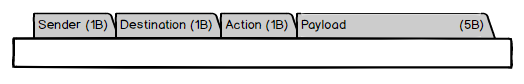
\includegraphics[width=\linewidth]{packet.png}
  \caption{Osnovna oblika paketa.}
  \label{fig:paket}
\end{figure}
Pošiljanje podatkov na radijskem modulu je omejeno na samo 8 bajtov na paket, zato sva pri implementaciji najine dodatne aplikacijske plasti poskušala čim več bajtov nameniti koristnim informacijam, saj bi to bilo v realni situaciji zaželeno. Prvi trije bajti so namenjeni naslavljanju paketkov ter funkcij Raft protokola in sicer: \\
\begin{itemize}
\item Prvi bajt je namenjen naslovu pošiljatelja paketka. Ta je pridobljen iz zadnjega ASCII znaka MAC naslova naprave.
\item Drugi bajt je namenjen naslova prejemnika paketka ("F" je broadcast).
\item Zadnji bajt identificira RAFT dejanje paketka.
\end{itemize}

Opis možne Raft vsebine: 
\begin{itemize}
\item A (ang. acknowledge) paket služi za potrditev prejema poljubnega sporočila, ter kot tip predstavitvenega paketa.
\item E (ang. election) paket poziva ostale naprave k glasovanju za novonastalega kandidata, ki je pošiljatelj paketa.
\item V (ang. vote) paket predstavlja glas privrženca, ki ga ta isti pošlje kandidatu in je odziv na E paket.
\item H (ang. heartbeat) paket ponastavi časovnik za nove volitve in ga pošlje vodja privržencem. V realnem svetu služi tudi za deljenje informacij med člani skupine (ang. log propagation).
\end{itemize} 


\begin{figure}
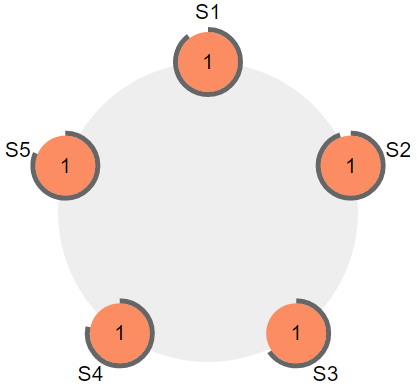
\includegraphics[scale=0.30]{raft_pics/raft1.png}
\end{figure}
\begin{figure}
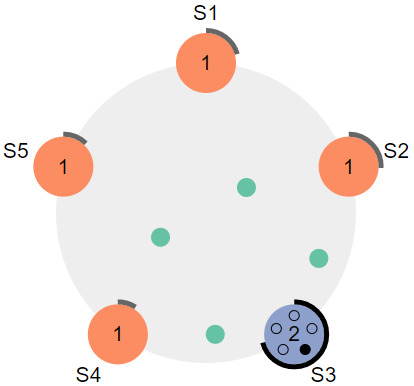
\includegraphics[scale=0.30]{raft_pics/raft2.png}
\end{figure}
\begin{figure}
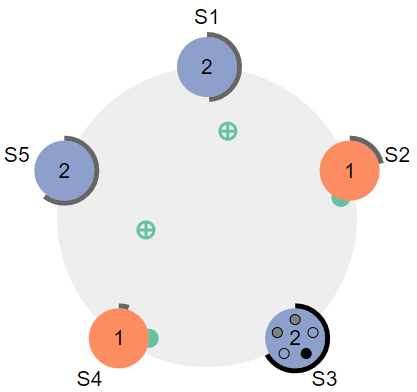
\includegraphics[scale=0.30]{raft_pics/raft3.png}
\end{figure}
\begin{figure}
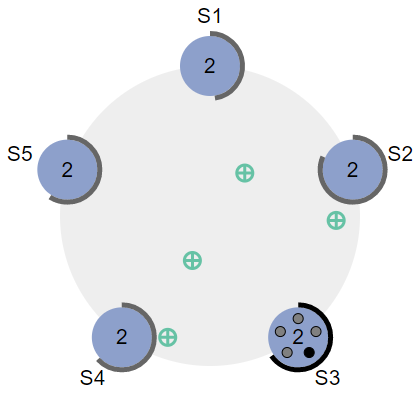
\includegraphics[scale=0.30]{raft_pics/raft4.png}
\end{figure}
\begin{figure}
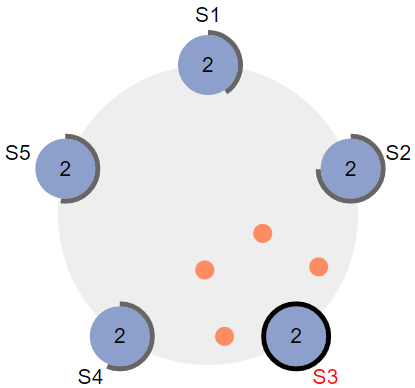
\includegraphics[scale=0.30]{raft_pics/raft5.png}
\caption{Shema tipičnega volitvenega cikla.}
\end{figure}

\section{Raft protokol}
Raft (Reliable ,Replicated ,Redundant, And Fault-Tolerant) je algoritem za sklepanje soglasja v porazdeljenih sistemih z več vozlišči. Narejen je bil leta 2014 z mislijo, da bo v veliki meri nadomestil starejši in veliko bolj zapleten Paxos algoritem. Omenjeno soglasje Raft doseže s pomočjo izvolitev vodilnega vozlišča. Naprava ima lahko v Raft skupini eno izmed treh vlog: \\
\begin{itemize}
\item Vodja (ang. leader)
\item Privrženec (ang. follower)
\item Kandidat (ang. candidate)
\end{itemize}
Odgovornost vodje je, da privržencem redno pošilja sporočila, da je ta še vedno aktiven (ang. heartbeat). Med tem ima vsak privrženec poljubni časovni interval (navadno med 150 ms - 300 ms), ki mu ob izteku spremeni vlogo v tisto kandidata ter sproži nove volitve. Če privrženec prejme potrditev, da je vodja aktiven pred iztekom časovnega intervala se ta ponastavi. 



\section{One time pad}
opis one time pad. zakaj smo si ga izbrali (ker je simple). opis kako bi se dalo razbit vsebino komunikacij. imam samo en stalen ključ, ker bi bilo ponovno izmenjevanje preveč zapleteno gleda na nivo fleksibilnosti, ki ga imamo v našem sistemu wemosov.
\section{Primeri}
\begin{figure}
  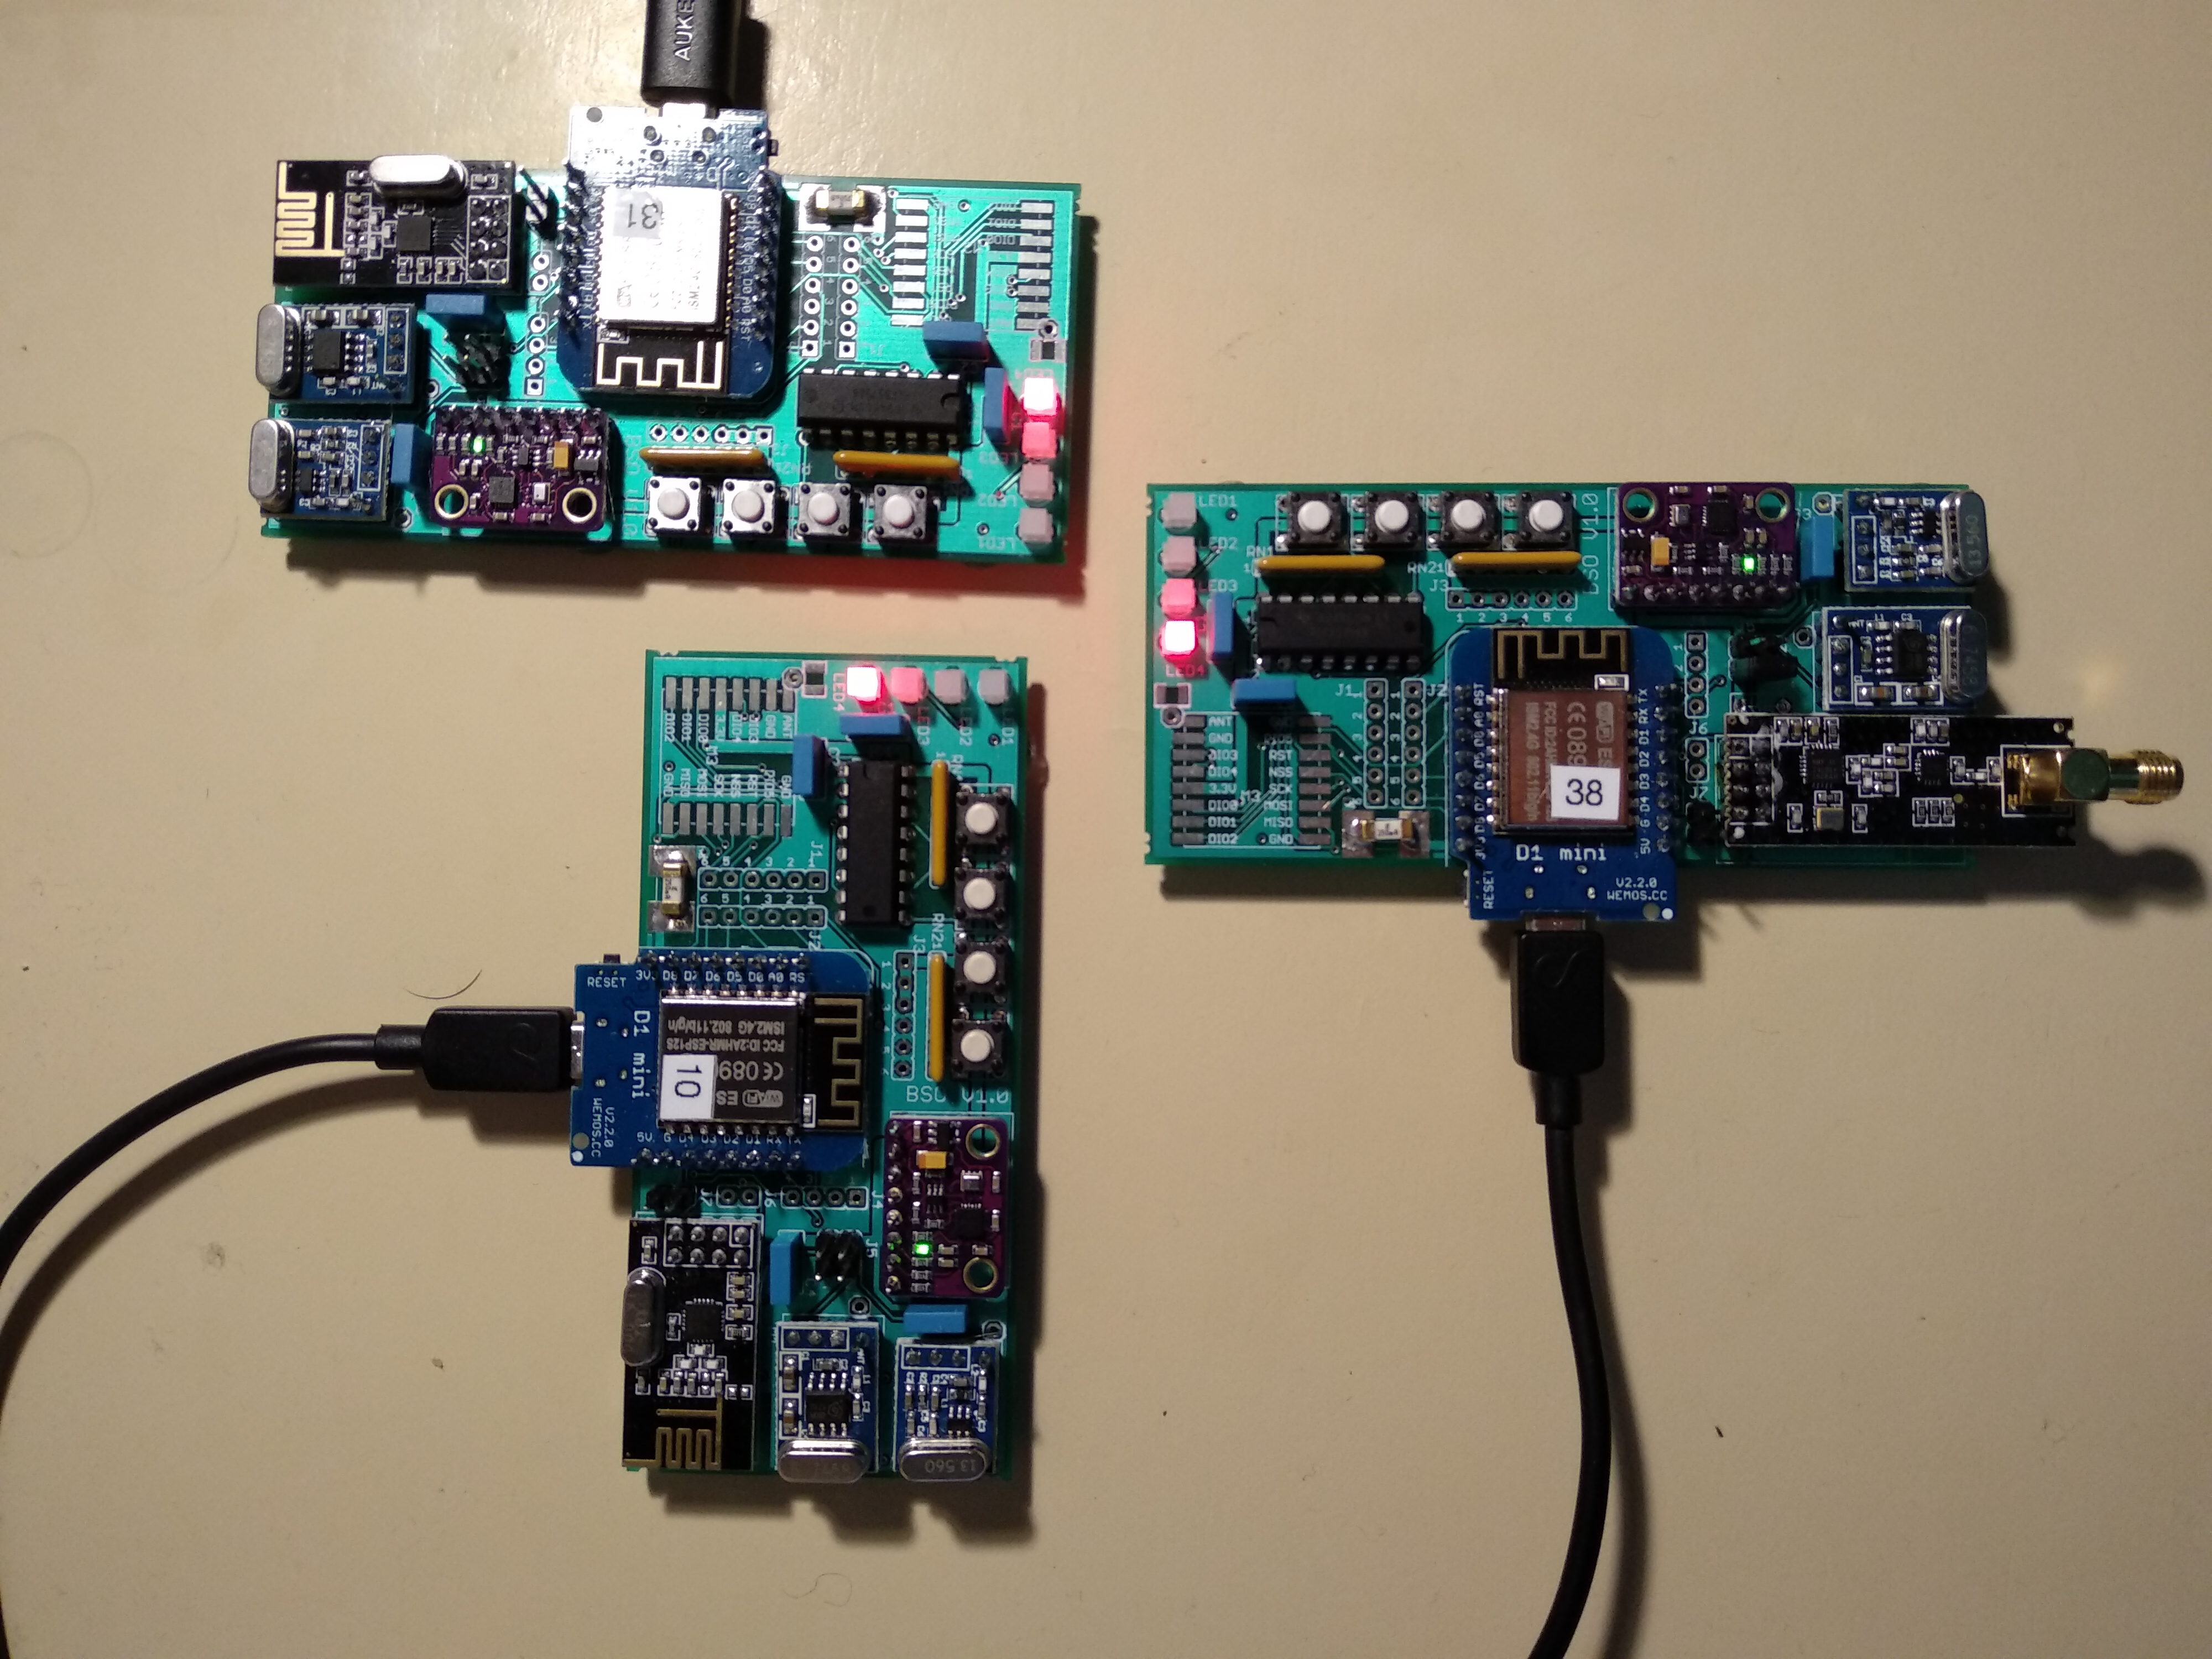
\includegraphics[width=\linewidth]{no_leader.jpg}
  \caption{Brez vodje bodo kmalu sledile nove volitve.}
  \label{fig:no_leader}
\end{figure}
\begin{figure}
  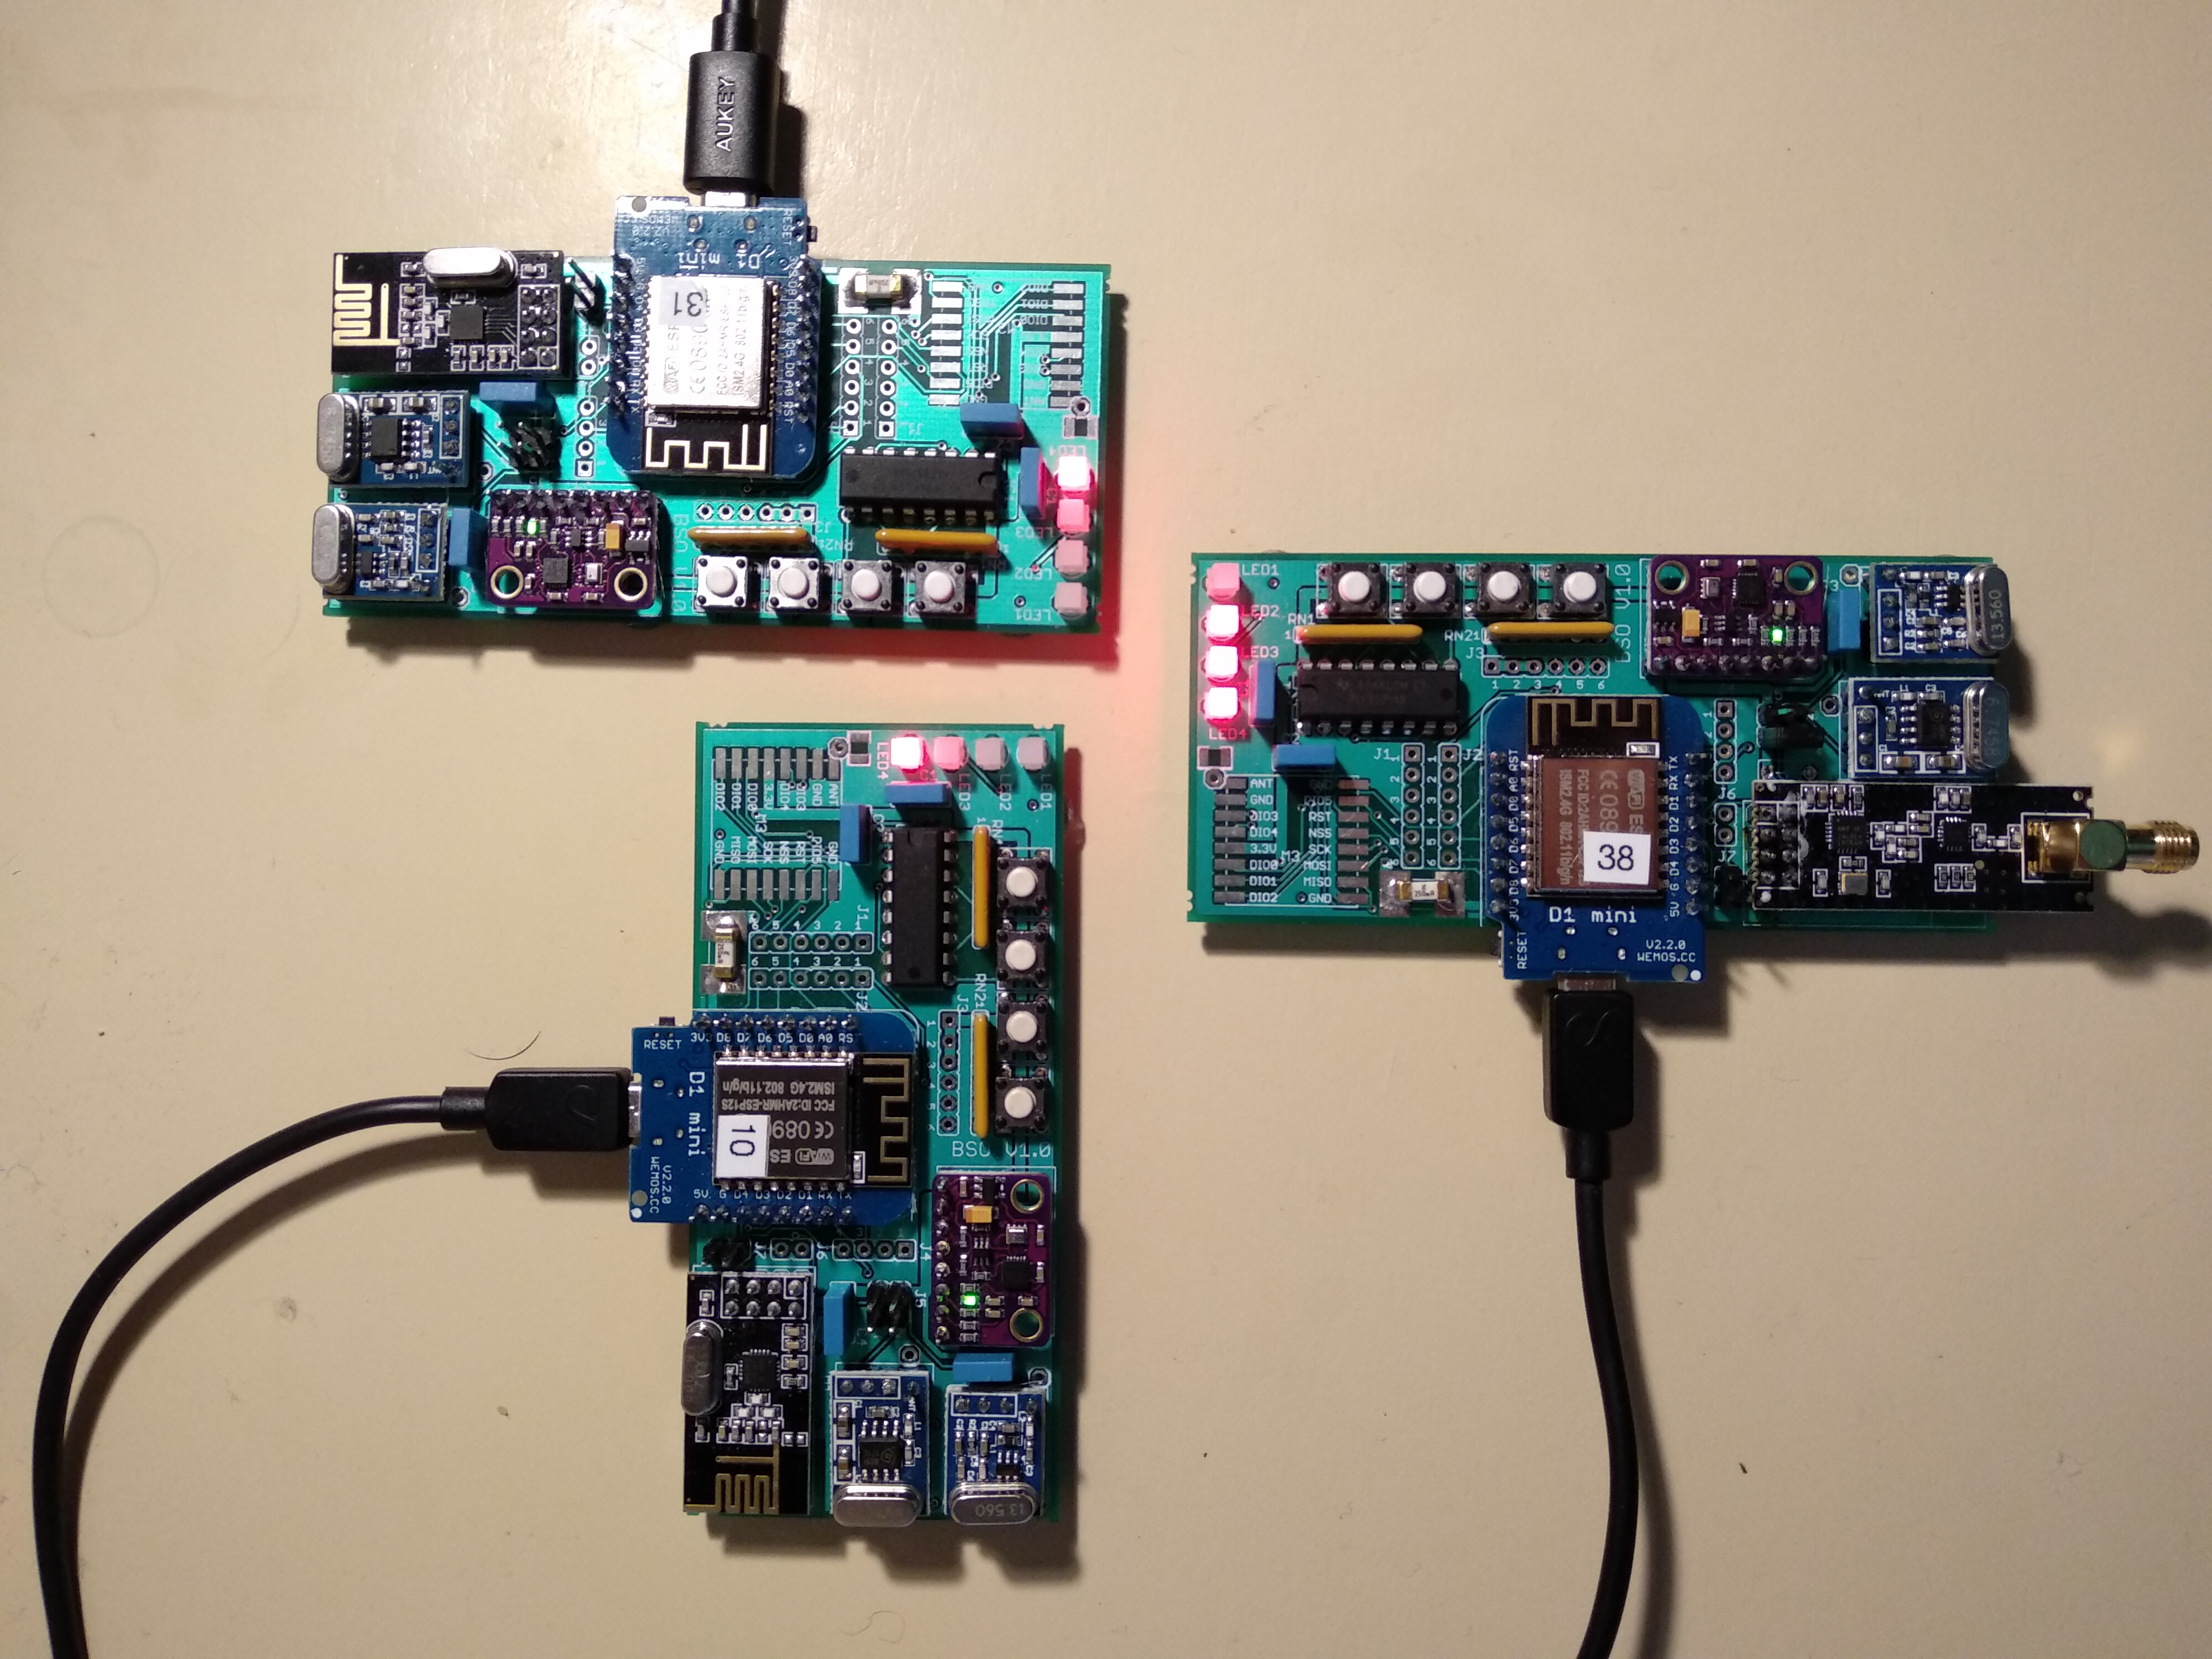
\includegraphics[width=\linewidth]{one_leader.jpg}
  \caption{Prisotnost vodje.}
  \label{fig:one_leader}
\end{figure}

\section{Zaključek}
dosežki projekta:
-delujoč določanje vodje (Raft)
-samo 1 preprosta koda za vsako napravo
-naprave se lahko poljubno priključijo v omrežje
-enkripcija one time pad
\end{document}

